\documentclass[a4paper,11pt]{article}
\usepackage[utf8x]{inputenc}
\usepackage[cm]{fullpage}
\usepackage{comment}
\usepackage{graphicx}

%opening
\title{475 - Advanced Topics in Software Engineering \\ Acme Telecom}
\author{Ramie Al-Omari \texttt{ra808}, Dan Cooke \texttt{dc408}, Jonathan Evans \texttt{je08}, Javad Moghisi \texttt{jm308}}

\begin{document}
\maketitle

Our client requested a minor modification to a simple, but vital mobile phone customer billing system; the current charging criteria charges customers peak rate for the entire duration of their call if any part of the call falls within a peak period. New regulations stipulate calls must be charged at peak rate only for the time spent within a peak period. This report examines our approaches and techniques used to safely modify and enhance the existing legacy codebase.

We quickly learned there was no documentation present (formal, tests or code comments). This presented us with a major problem; an unknown existing system specification. The requirements specified that other than the stipulated modification, all other functionality should remain unchanged. Clearly the existing functionality would need to be accurately specified to ensure this condition is met. Thus our first goal was to develop a clear specification of the existing system, to allow us to safely refactor the codebase.

We began by implementing a Runner class with a main method to exercise various functionality within the system. The initial workload was split between the group into writing acceptance tests using the FitNesse framework, writing integration tests with JUnit and setting up a developer workflow including build and dependency management as well as a continuous integration server.

We assumed that the deadline for delivering the functionality to comply with the new regulations, coincides with the coursework submission deadline. Therefore our first priority was to ensure that these requirements would be met in a safe and timely manner.
\begin{comment}
Understanding the specified requirements.
Reading spec
Clarifying with client
writing up requirement list
New requirements.
listening to customers and domain experts
\end{comment}

\section{Acceptance Testing}
To specify the functionality of the new system we wrote acceptance tests that captured both the new requirements and the remaining, unchanged behaviour of the old system. As there was no formal specification we had to be careful that these captured the full behaviour of the system. The tests we implemented specified the following behaviour:

Calls that:
\begin{itemize}
\item start and finish during the same peak time range
\item start and finish during the same off peak time range
\item start during a peak time range and finish at the following off peak time range
\item start during an off peak time range and finish at the following peak time range
\item start during one off peak time range and finish at the following off peak time range
\item start during one peak time range and finish at the following peak time range
\end{itemize}

We implemented the acceptance tests using Fit documents and executed them using the FitNesse acceptance testing framework. We decided to use Fit documents to specify the system as they can easily be edited and read by non-technical stakeholders at AcmeTelecom. FitNesse allows AcmeTelecom to modify, view and run the tests from a user friendly wiki interface. 

Our Fit documents followed the Given When Then structure popular in behaviour driven development. It allowed us to form behaviour "narratives" that used domain language in a natural way that the client can understand. Also most of our tests were data driven and the Given section permitted us to easily specify the information required by the test.  
\\

An example of Fit test can be seen below:

\begin{center}
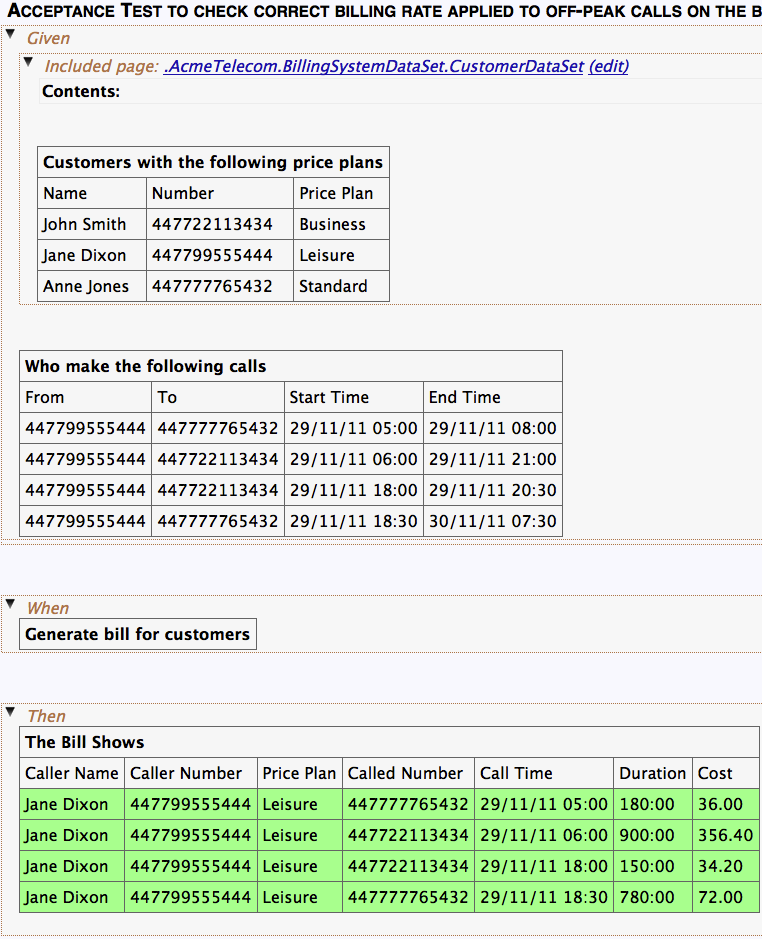
\includegraphics[scale=0.5]{images/fitnesse_test.png}
\end{center}



\section{Unit Testing}

We implemented a comprehensive passing integration tests to prevent us from breaking existing functionality as we refactored the code base. This was particularly tricky as the createCustomerBills method of BillingSystem output to stdout. The test would set up a number of calls before requesting the bill for those customers. In order to check the output bill we had to redirect Sys.out to a PrintStream, collecting the generated bill into a string on which assertions could be made.

The existing system had not been written with testing in mind so it was very difficult for us to write unit tests or wire up our FitNesse tests. In order to introduce new unit tests we needed to introduce seams enabling us to isolate sections of code. The seams were necessary to break dependencies and allow injection of test values. For example, as the system used the current system time for logging calls, we couldn't create repeatable, non-brittle tests. With the integration tests in place we were confident in refactoring the code to allow arbitrary times to be injected into CallEnd and CallStart.

\begin{verbatim}
public CallEnd(String caller, String callee, long timestamp) {
    super(caller, callee, timestamp);
}
\end{verbatim}

After making these changes we ensured that the integration test continued to pass and started implementing new functionality using Test-Driven Development (TDD).  As we broke dependencies we introduced interfaces which could be mocked and allowed for testing and verification of object interactions. 

For our unit testing framework we used JUnit assisted by Mockito for mocking objects and EMMA for gathering code coverage statistics. Upon completion of the project we had 92\% code coverage

\begin{comment}
Important to get good code coverage and high quality tests which test edge cases such e.g. getting the time of the next off peak / peak change
calls that last for less than a second - keep the behaviour the same but consult with the client f there is a m
self documenting
HAMCREST and dsl
Requirement analysis.
clear document of requirements filtering non essential information
analysis
remote debugging of fitnesss using eclipse
\end{comment}


\section{Refactoring}
The old code was an unorganised 'big ball of mud' that had many cyclic dependencies and no clear layering. This meant that adding functionality requires changing code across the whole code base and made it difficult to for us to build acceptance tests and unit tests as we couldn't inject the required mock objects. Another issue is that the code was not organised into packages, making it difficult to locate relevant code.  We made the following steps to remedy these problems:
\begin{itemize}
\item After initial analysis it became clear that acceptance testing on the initial codebase would be challenging; the functionality is centered around time instances which are not injected, making mocking difficult. We decided to inject the timestamp from a higher level so the timestamp could be mocked. This allowed us to implement basic acceptance tests to verify overall system behavior under different call time scenarios.
\item We decided to remove call logging responsibility from BillingSystem with the intention of injecting an interface that supports call retrieval, this would allow much greater flexibility as the way calls are logged is now completely separated from the BillingSystem.
\item Clearly the call events must now be injected into a call log instance, the actual implementation is similar to the previous BillingSystem implementation but now injects the timestamp as described in the first point. 
\item An overridden method was introduced into the CallEvent class to remove the 'instanceof' usage in the call calculation method.
\item TarrifLibrary and CustomerDatabase interfaces are now injected into BillingSystem to remove implementation dependency, this is a crucial step as mocking can now be used to unit test BillingSystem.
\item A BillGenerator interface is injected into BillingSystem, this allows control over the BillGenerator type (e.g. to allow different formatting options).
\item To finalise the refactoring of BillingSystem, the call cost functionality is now injected via an interface to allow for greater flexibility, the old calculation method can easily be swapped for new calculation methods for example, this will be particularly useful later for acceptance testing. Also a BillItem abstract server was introduced to remove the reverse dependency from Printer.
\end{itemize}

Components.- irrelevant?
If its got manual DI its probably been made into compopnents 
Dependency injection frameworks (e.g. Guice or Spring) - not yet but guice

http://www.natpryce.com/articles/000783.html
we thought about 2 phone calls at the same time with the same people 
Dependency principles.


The structure before and after refactoring are shown below:
%Diagram before
\begin{center}
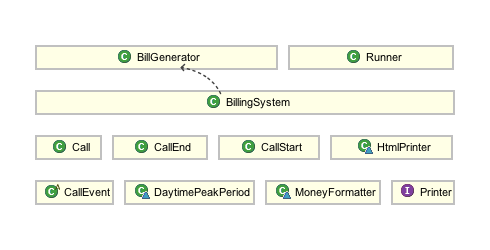
\includegraphics[scale=0.75]{images/original_structure.png}
\end{center}

<CHECK BEFORE SUBMISSION>

Clearly the structure has been much improved, the new layering enables much greater configurability.
different billing methods fairly easily without impacting other packagers. All of the logic for calculati

\begin{verbatim}
public void createCustomerBills(Log callLog) {
    for (Customer customer : customerDatabase.getCustomers()) {
        createBillFor(customer, callLog);
    }
}

private void createBillFor(Customer customer, Log callLog) {
    BigDecimal totalBill = new BigDecimal(0);
    List<BillItem> items = new ArrayList<BillItem>();
    Tariff tariff = tariffLibrary.tarriffFor(customer);
    for (Call call : callLog.getCalls(customer)) {
        BigDecimal callCost = billCalculator.getCallCost(tariff, call, peakPeriod);
        totalBill = totalBill.add(callCost);
        items.add(new LineItem(call, callCost));
    }
    billGenerater.generate(customer, items, totalBill);
}
\end{verbatim}
\begin{comment}

TODO FILE

concentrate on understanding where rule is defined in existing system
add main method and run application
write acceptance test for existing behaviour, ensures that using latest working code base
code not written with testing in mind, can't wire up acceptance tests easily/correctly
needs refactoring in order to be able to sense values, inject customers/calls and remove dependency on current time (brittle tests)
create seam/inject it, but don't want to do that without refactoring code before writing test,
so change it so the code always uses a fixed time, write unit tests for safety net, refactor time out and use mock for tests
acceptance tests done against real database, need to use DI and mock implementation so get predictable tests
verify requirements with user, bridge communication gap using Cucumber
once verified existing code is actually working, can almost 'discard' those tests and create acceptance tests for new behaviour
when is the deadline for this new regulation? assumption that is at cw submission deadline
implement new rule, make sure this requirement is met first, don't throw away existing code!
then concentrate on refactoring design for extensibility under safety of

Acceptance Tests
	gather requirements from user
	fit/cucumber tests
TDD
	introduce seams,
	unit tests, (EMMA code coverage)
Object-Oriented
	objects have roles
	tell, don't ask
	mock objects (mockito)
	Ports and Adapters
DSL?
	domain driven
	fluent interface
	guide the API user
layering (structure 101)
	interfaces for abstractions
	abstract server/client
	interface segregation principle
dependency injection (google guice)
	handling singletons
	frameworks?
developing under pressure
	iterative development
	requirements analysis and design
	develop a feature at a time (vertical slice)
	extend with extra functionality (horizontal slice)
deployment/release
	continuous integration (jenkins)
	continuous deployment after implementing basic requirements
	blue/green, canary, split test, (production parallel)

jbehave
jenkins/cucumber on micro EC2 instance
build and dependency management using buildr/gradle
build management using or gant
issue tracking tools e.g. JIRA
adding a UI or designing bills e.g. balsamiq mockups

different way of showing the bill/receipt
rules could change in the future
use JodaTime


off-peak charges (pence/minute):
standard: 0.12
business: 0.18
leisure: 0.06

peak charges (pence/minute):
standard: 0.30
business: 0.18
leisure: 0.48

bill shows how portion of call was charged
from 7th hour onwards changes tariff
still using existing peak off-peak function
order calls by start time then duration on the bill!
acceptance tests across call plans use the same call times (control/fairness/clearness)
query table for call costs, split per customer
test 0.04 seconds, currently not charged

wrote a nearly end-to-end FitNesse test
had to redirect System.out!
fixed the times!
failed on jenkins due to newline char being different, so disabled it on CI, but still passed locally
introduced seam, changed so that call time could be injected into call event, able to test
gets tariff for each customer inside call loop, inefficient, call it from outside
injected billgenerator
created new test using mocking of billgenerator, customerdb, tarifflib
billgenerator does not need string totalBill as lineitems has this already! move calc total bill to billgenerator
still use callinit and call complete, still with fixed times
but needed to add equals and hashcode to lineitem, call, callevent for verifying billgen send, also better than comparing primitives
added tests for equals in lineitem, call, callevent
broke up createBillForCustomer into a number of methods such as getCallsFor(customer), calculateCostOfEachCall, calculateTotalBill, able to sense values
introduce CallLogger with getCallsFor(customer)
noticed calls are synchronous, system doesn't allow simultaneous calls, need to check requirements but kept behaviour the same, added test to check this
callLogger injected into BillingSystem, e.g. can have async call logger
separate out BillCalculator
tests for BillCalculators only used one of the tariffs, the acceptance test cover all cases
add Fixed (old requirements) and Variable (new requirements) calculator
peakperiod logic unchanged, injected into calculator
// todo: BillCalculator use setter injection and default to variable rate!
refactored structure into three main packages (billing, calls, printing), removed cyclic dependency between billsystem and billgenerator
billgenerator not ordered, check requirements with user
integration test for BillGenerator used HtmlPrinter, again redirect sysout, refactored to inject dependency, removed the totalCost argument
Customer builder with tinytypes for firstname, lastname, number
CallEvent builder with tinytypes

findbugs
jdepend?

ports and adapters, especially around the customer and tariff db!!
CallEvent map?


for DSLs we used mockito, joda time, hamcrest, our own, suggest one for query CallLogger
=======
findbugs
jdepend?


The current code was an unorganised �big ball of mud� that had many cyclic dependencies meaning that adding functionality requires changing code across multiple classes making it difficult to prevent errors and test rigorously. Another issue is that the code was not organised into packages...So prior to adding the new functionality we organised the classes into packages then analysed the current code using structure 101 to locate these cyclic dependencies. We obtained the following graph:


The risk is that the code becomes a �big ball of mud� that is difficult to understand. Extending such as system requires that many classes and test be modified across multiple packages.

The requirements we were given meant that vertical slicing was not plausible as we essentially only needed to modify the implementation of one horizontal slice. However
Domain Specific Languages.
Dependency inversion: abstract client and abstract server (in code refactoring)
Dependency injection
Modularity and Layering.
The top of a hierarchy can be easily changed as there aren�t any incoming dependencies.
Slicing
vertical slicing??? - not really relevant

\end{comment}


%Diagram after

%Wrote new code
\section{Implementing Variable Billing}
As the refactoring has given us an interface "BillCalculator", we can add ng the price can be done in one function, "getCallCost" in the implementation of BillCalculator.

We have decided to make use of Joda-Time for storing call start times and end times, as this class has a lot of useful functions for making calculations with dates.

\begin{verbatim}
public BigDecimal getCallCost(Call call, Tariff tariff, DaytimePeakPeriod peakPeriod) {
    DateTime currentTime = call.startTime();
    DateTime endTime = call.endTime();
    int totalOffPeakDuration = 0;
    int totalPeakDuration = 0;
    while (currentTime.compareTo((call.endTime())) < 0) {
        DateTime nextPeakChange = peakPeriod.nextPeakChange(currentTime);
        int peakDuration = Math.min(Seconds.secondsBetween(currentTime,          endTime).getSeconds(),
        Seconds.secondsBetween(currentTime, nextPeakChange).getSeconds());
        if (peakPeriod.offPeak(currentTime)) {
            totalOffPeakDuration += peakDuration;
        } else {
            totalPeakDuration += peakDuration;
        }
        currentTime = currentTime.plusSeconds(peakDuration);
    }
    BigDecimal offPeakCost = new BigDecimal(totalOffPeakDuration).multiply(tariff.offPeakRate());
    BigDecimal peakCost = new BigDecimal(totalPeakDuration).multiply(tariff.peakRate());
    return offPeakCost.add(peakCost).setScale(0, RoundingMode.HALF_UP);
}
\end{verbatim}

We made us of a new function "nextPeakChange" which given a time, returns the following time boundary between on and off peak. This means we can work out at most how long they should be charged at a given rate in O(1) time.

The code works by starting from the beginning of the call and adding the number of seconds between the current time and the next boundary to either th5e off peak duration or on peak duration. It then continues to do this from the previous boundary until the end. This function has a complexity of O(k) where k is the number of boundaries. As we can assume no conversation lasts over 24 hours, we will only loop at most 3 times.

\begin{comment}
With the new organisation of the code we have seperate classes for the old and new billing methods:
FixedRateBillCalculater and VariableRateBillCalculater so that we could have unit tests for both.

Made use of Joda-Time instead of the current DateTime library as it has extra functionality.
DSL JODA TIME + mockito AND HAMCREST

Once the code was refactored, we simply needed to implement one function in the FixedRateBillCalculater (all the logic in the same place)			
does the minute at the peak boundary count as on peak or off peak
\end{comment}

%Anything else you did
\section{Development Process}
We used the GIT distributed version control system to allow our team to effectively collaborate on the same code, hosting our repository on Github as they offer a reliable service and free accounts for students. Using a free micro instance on Amazons Elastic Compute Cloud (EC2) we set up the free Jenkins Continuous Integration (CI) system. Every commit to git would trigger Github's post web hooks, alerting Jenkins that there had been a commit. Jenkins would then checkout the code, build it, run the acceptance tests using FitNesse, integration tests and unit tests using JUnit, and generate code coverage with EMMA. We could also see the status of the builds of all commits along with their code coverage and test status using the Jenkins web interface shown below. Every time the build status changed, i.e. a successful build after a failed build of a failed build after a successful build, and email would be sent to the group as a warning. Using continuous integration enabled the group to track our progress towards a system with full code coverage and then ensure that we maintained the coverage as we made changes. Utilising CI added momentum to the development process as we all wanted full code coverage and to keep the build green. Below is a screenshot of the project page on Jenkins web interface with testing and code coverage graphs.

To manage building and other tasks associated with the project we used Gradle. We used Gradle as it has a good domain model for build tasks and is very flexible, allowing you to use both ant/Maven build tasks and maven repositories if required. Java build targets were set up by simply including the java plugin although we had to add a main class attribute to the jar manifest file. We also used the emma plugin so that every time we built the test task, EMMA code coverage statistics were generated for Jenkins to use. Lastly we used the idea plugin, this allowed us to generate Intellij IDEA project files which had the libraries and build targets as defined in the Maven build. 

To deploy the system we would extend the current continuous integration system to automatically promote the new builds to production. As this is a desktop application and not a web app, production could correspond to a versioned folder with a symlink to the latest version (to allow blue/green releasing) or a update system to push the software to the users.

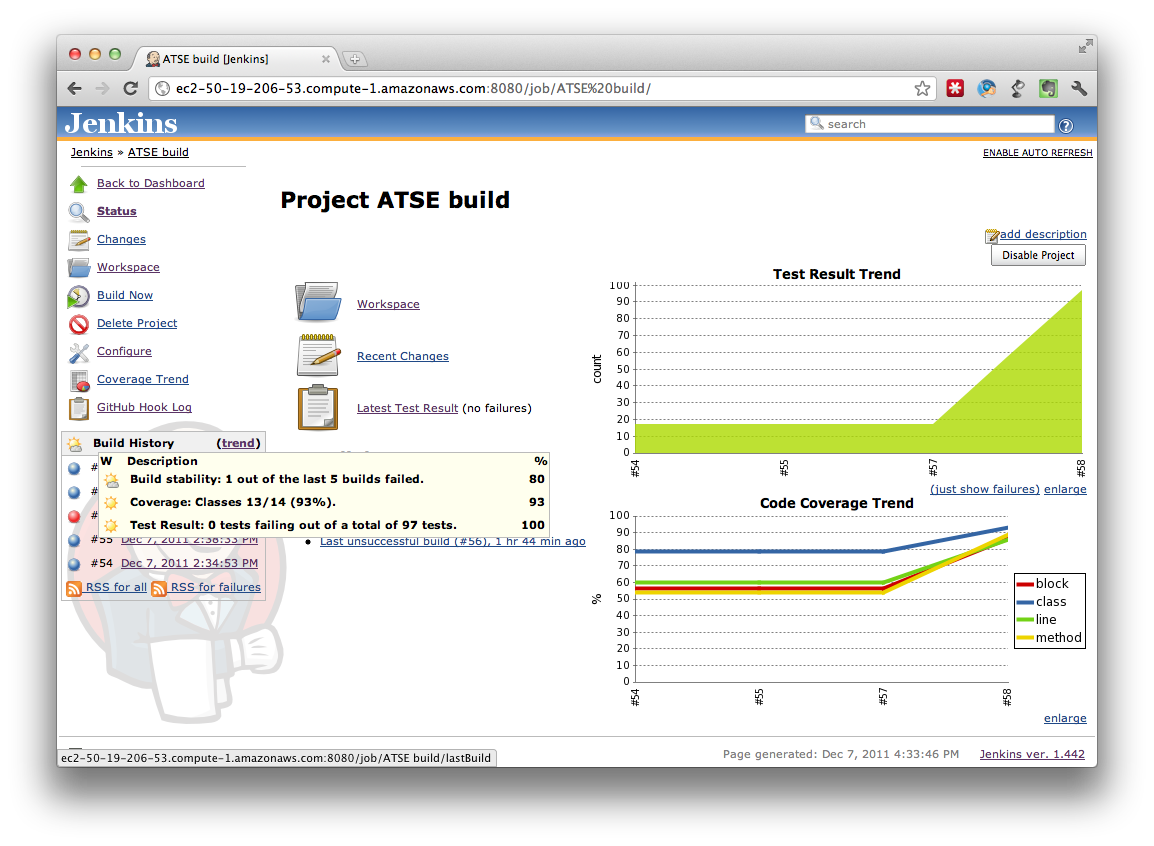
\includegraphics[scale=0.4]{images/jenkins_project.png}

%\section{Something else}

% Managing future improvements
\section{Future Improvements}
Managing future improvements
Concurrent calls.
Call ordering on bill. 
Extend continuous integration to allow continuous deployment.
nice examples of when to 
gen call for bill that hasn't endend

\end{document}